

\tikzset{every picture/.style={line width=0.75pt}} %set default line width to 0.75pt        

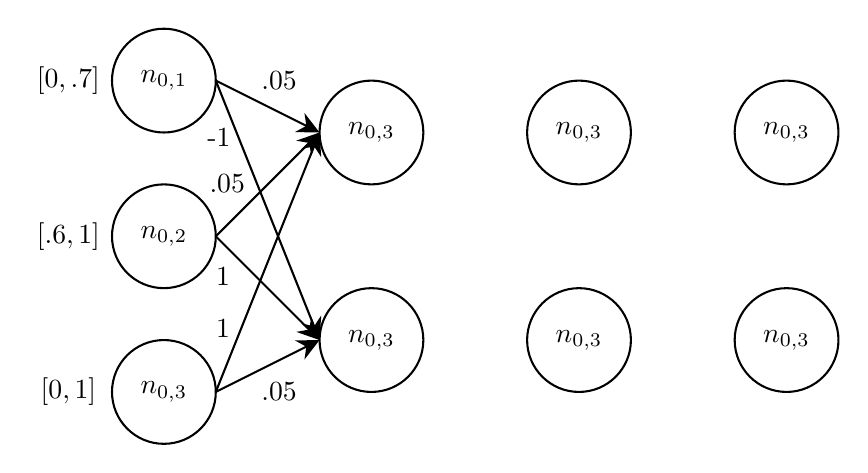
\begin{tikzpicture}[x=0.75pt,y=0.75pt,yscale=-1,xscale=1]
%uncomment if require: \path (0,394.8000030517578); %set diagram left start at 0, and has height of 394.8000030517578

%Shape: Circle [id:dp34241330653932067] 
\draw   (75,175) .. controls (75,161.19) and (86.19,150) .. (100,150) .. controls (113.81,150) and (125,161.19) .. (125,175) .. controls (125,188.81) and (113.81,200) .. (100,200) .. controls (86.19,200) and (75,188.81) .. (75,175) -- cycle ;
%Shape: Circle [id:dp41065166902904626] 
\draw   (75,100) .. controls (75,86.19) and (86.19,75) .. (100,75) .. controls (113.81,75) and (125,86.19) .. (125,100) .. controls (125,113.81) and (113.81,125) .. (100,125) .. controls (86.19,125) and (75,113.81) .. (75,100) -- cycle ;
%Shape: Circle [id:dp40483783964492026] 
\draw   (75,250) .. controls (75,236.19) and (86.19,225) .. (100,225) .. controls (113.81,225) and (125,236.19) .. (125,250) .. controls (125,263.81) and (113.81,275) .. (100,275) .. controls (86.19,275) and (75,263.81) .. (75,250) -- cycle ;
%Shape: Circle [id:dp46268332512914756] 
\draw   (175,225) .. controls (175,211.19) and (186.19,200) .. (200,200) .. controls (213.81,200) and (225,211.19) .. (225,225) .. controls (225,238.81) and (213.81,250) .. (200,250) .. controls (186.19,250) and (175,238.81) .. (175,225) -- cycle ;
%Shape: Circle [id:dp37297033939244173] 
\draw   (175,125) .. controls (175,111.19) and (186.19,100) .. (200,100) .. controls (213.81,100) and (225,111.19) .. (225,125) .. controls (225,138.81) and (213.81,150) .. (200,150) .. controls (186.19,150) and (175,138.81) .. (175,125) -- cycle ;
%Straight Lines [id:da8339229391161269] 
\draw    (125,100) -- (172.32,123.66) ;
\draw [shift={(175,125)}, rotate = 206.57] [fill={rgb, 255:red, 0; green, 0; blue, 0 }  ][line width=0.08]  [draw opacity=0] (10.72,-5.15) -- (0,0) -- (10.72,5.15) -- (7.12,0) -- cycle    ;
%Straight Lines [id:da2911234225445125] 
\draw    (125,100) -- (173.89,222.21) ;
\draw [shift={(175,225)}, rotate = 248.2] [fill={rgb, 255:red, 0; green, 0; blue, 0 }  ][line width=0.08]  [draw opacity=0] (10.72,-5.15) -- (0,0) -- (10.72,5.15) -- (7.12,0) -- cycle    ;
%Straight Lines [id:da24815609644474668] 
\draw    (125,175) -- (172.88,127.12) ;
\draw [shift={(175,125)}, rotate = 495] [fill={rgb, 255:red, 0; green, 0; blue, 0 }  ][line width=0.08]  [draw opacity=0] (10.72,-5.15) -- (0,0) -- (10.72,5.15) -- (7.12,0) -- cycle    ;
%Straight Lines [id:da6811832588192949] 
\draw    (125,250) -- (172.32,226.34) ;
\draw [shift={(175,225)}, rotate = 513.4300000000001] [fill={rgb, 255:red, 0; green, 0; blue, 0 }  ][line width=0.08]  [draw opacity=0] (10.72,-5.15) -- (0,0) -- (10.72,5.15) -- (7.12,0) -- cycle    ;
%Straight Lines [id:da84952601885845] 
\draw    (125,175) -- (172.88,222.88) ;
\draw [shift={(175,225)}, rotate = 225] [fill={rgb, 255:red, 0; green, 0; blue, 0 }  ][line width=0.08]  [draw opacity=0] (10.72,-5.15) -- (0,0) -- (10.72,5.15) -- (7.12,0) -- cycle    ;
%Straight Lines [id:da7046423339728956] 
\draw    (125,250) -- (173.89,127.79) ;
\draw [shift={(175,125)}, rotate = 471.8] [fill={rgb, 255:red, 0; green, 0; blue, 0 }  ][line width=0.08]  [draw opacity=0] (10.72,-5.15) -- (0,0) -- (10.72,5.15) -- (7.12,0) -- cycle    ;
%Shape: Circle [id:dp13563446564676784] 
\draw   (275,225) .. controls (275,211.19) and (286.19,200) .. (300,200) .. controls (313.81,200) and (325,211.19) .. (325,225) .. controls (325,238.81) and (313.81,250) .. (300,250) .. controls (286.19,250) and (275,238.81) .. (275,225) -- cycle ;
%Shape: Circle [id:dp818022405634492] 
\draw   (275,125) .. controls (275,111.19) and (286.19,100) .. (300,100) .. controls (313.81,100) and (325,111.19) .. (325,125) .. controls (325,138.81) and (313.81,150) .. (300,150) .. controls (286.19,150) and (275,138.81) .. (275,125) -- cycle ;
%Shape: Circle [id:dp8652117882296453] 
\draw   (375,125) .. controls (375,111.19) and (386.19,100) .. (400,100) .. controls (413.81,100) and (425,111.19) .. (425,125) .. controls (425,138.81) and (413.81,150) .. (400,150) .. controls (386.19,150) and (375,138.81) .. (375,125) -- cycle ;
%Shape: Circle [id:dp8104123077273672] 
\draw   (375,225) .. controls (375,211.19) and (386.19,200) .. (400,200) .. controls (413.81,200) and (425,211.19) .. (425,225) .. controls (425,238.81) and (413.81,250) .. (400,250) .. controls (386.19,250) and (375,238.81) .. (375,225) -- cycle ;

% Text Node
\draw (54,100) node    {$[ 0,.7]$};
% Text Node
\draw (54,175) node    {$[ .6,1]$};
% Text Node
\draw (54,250) node    {$[ 0,1]$};
% Text Node
\draw (100,100) node    {$n_{0,1}$};
% Text Node
\draw (100,175) node    {$n_{0,2}$};
% Text Node
\draw (100,250) node    {$n_{0,3}$};
% Text Node
\draw (155.5,100) node  [font=\normalsize] [align=left] {.05};
% Text Node
\draw (126.5,127.5) node  [font=\normalsize] [align=left] {\mbox{-}1};
% Text Node
\draw (130.5,149.5) node  [font=\normalsize] [align=left] {.05};
% Text Node
\draw (128.5,194.5) node  [font=\normalsize] [align=left] {1};
% Text Node
\draw (128.5,219.5) node  [font=\normalsize] [align=left] {1};
% Text Node
\draw (155.5,250) node  [font=\normalsize] [align=left] {.05};
% Text Node
\draw (200,225) node    {$n_{0,3}$};
% Text Node
\draw (200,125) node    {$n_{0,3}$};
% Text Node
\draw (300,225) node    {$n_{0,3}$};
% Text Node
\draw (300,125) node    {$n_{0,3}$};
% Text Node
\draw (400,125) node    {$n_{0,3}$};
% Text Node
\draw (400,225) node    {$n_{0,3}$};


\end{tikzpicture}
